\setcounter{page}{1}
\begin{center}
    \heiti \zihao{3}基于机器学习的车位规划\\
    开题报告
\end{center}
\songti \zihao{-4}
\section{选题背景与意义}
\subsection{选题背景}
随着我国经济社会的快速发展,人们的生活水平显著提高,汽车保有量的持续呈现增长趋势。据中国汽车工业协会数据显示,2023年汽车产销分别完成3016.1万辆和3009.4万辆,同比分别增长11.6\%和12\% (如图\ref{fig:cars_sales})。这表明汽车在我国的普及和使用呈现出强劲的发展态势。
\begin{figure}[H]
  \centering
  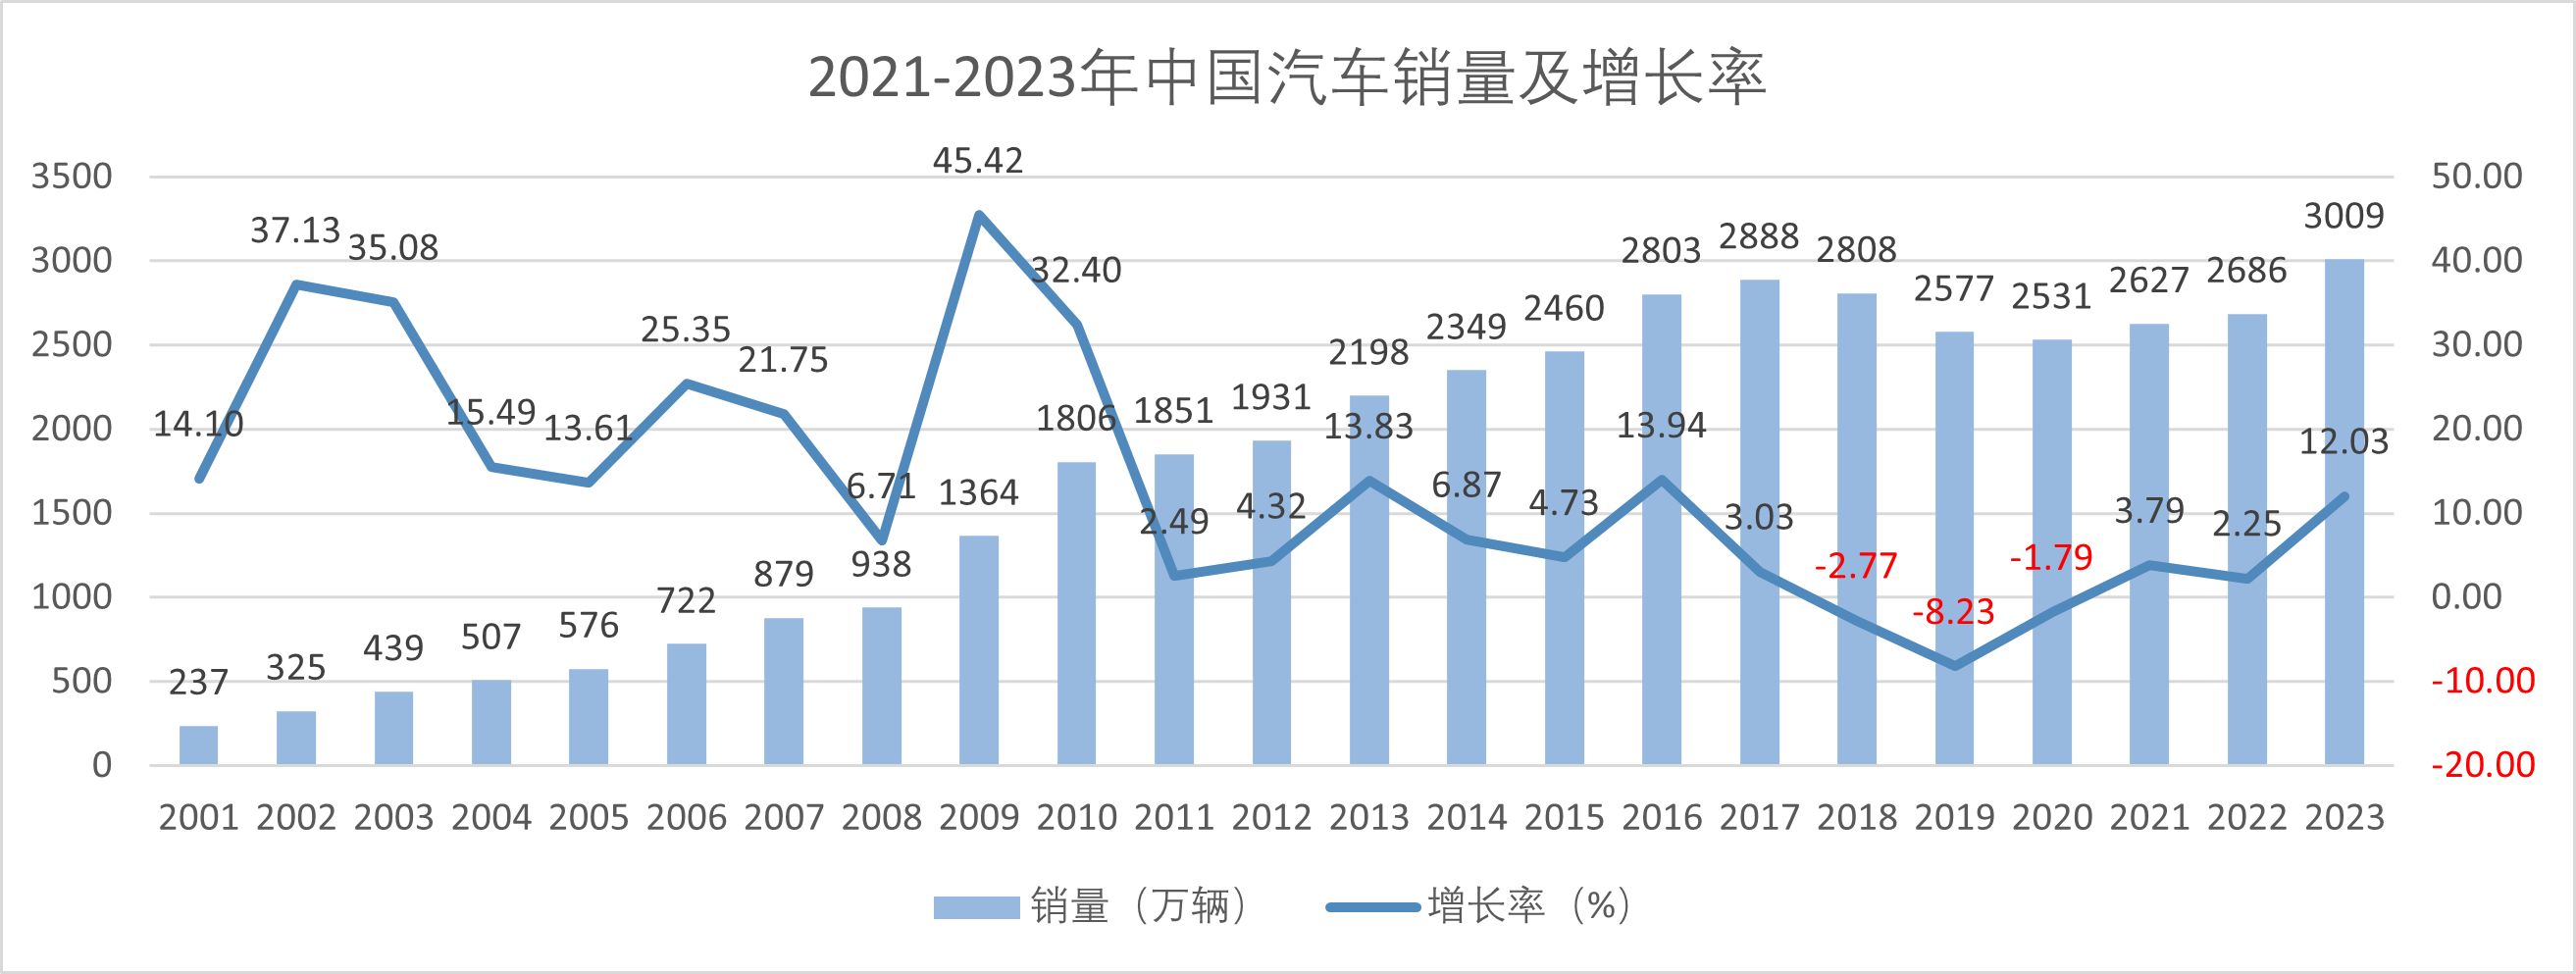
\includegraphics[width=0.7\textwidth]{pictures/2021-2023年中国汽车销量及增长率.png}
  \caption{2021-2023年中国汽车销量及增长率}
  \label{fig:cars_sales}
\end{figure}
随着城镇化进程加速\cite{XXCZ202306017},城市密度激增\cite{JZXB201004006},土地资源紧缺问题逐渐凸显。而在这种情况下,人们对于汽车的购买欲望提升,车辆的增加虽然带来了便捷的生活,但也造成了交通系统压力大、停车基础设施不足等问题\cite{CSDQ200708009},如何充分利用停车资源、开发地下停车场\cite{JSSD201905002}并增加经济效益等成为当前城市发展的紧迫问题。

其中,建造地下停车场是一种极为有效的解决方案。同等土地面积下,相较于传统的露天停车场,地下停车场能够提供更多的停车位\cite{1022811825.nh},同时也能节省城市建设用地。此外,地下车库还能有效地缓解地面动静态交通矛盾\cite{CSDQ201807120}。虽然地下车库有诸多优点,但仍存在以下问题:
\begin{enumerate}
    \item {\bfseries 规范不统一。}各个公司均用私有规范,导致产生行业壁垒,行业无法快速进步。
    \item {\bfseries 设计参数多。}除去政策、法律等规定的固定参数\cite{ZGBZ202119043},还包含了一些不容建筑公司定制化的可变参数。
    \item {\bfseries 结构复杂。}相较于地上停车场,地下停车场结构更为复杂。
\end{enumerate}
以上原因,均加剧了地下车库设计远远落后于地上的情况。

在大量建设地下停车场的同时,由于设计师的设计流程较为耗时,未能满足开发商对于周期、质量等的成本要求,因此他们将目光转移到了“一键式”生成设计图。与此同时,Autodesk\cite{carrasco2005innovative,JCJG202304039}等公司开发了一款适用于建筑行业的设计软件AutoCAD,为设计师进行图纸修改提供了更便捷的方式。

基于以上背景,我们致力于设计和开发基于强化学习的车位自动化排布算法并进行可视化展示。
\subsection{选题意义}
\subsubsection{现实意义}
\begin{itemize}
    \item {\bfseries 减轻设计压力。}大幅缩短设计师的设计流程,简化一些较为简单的设计,减少低效的重复劳作。
    \item {\bfseries 提供多种方案。}针对同一初始场地,可利用不同算法进行设计,可能会出现不同的排布方案,便于设计师进行选择。
    % \item {兼容不同参数。}当某一参数改变时,可仅通过改变输入尺寸重新计算来进行修改,而不需要设计师从头排列设计。
    \item {\bfseries 降低修改成本。}面对一些特殊情况,如需求改变、车位尺寸改变等,只需付出较少的成本便可重新设计和布局。
    % 算力换多种指标衡量 前端页面展示的数据 供用户使用 给个更改奖励的接口
\end{itemize}
\subsubsection{技术意义}
\begin{itemize}
    \item {\bfseries 跨学科融合。}通过将一个较为复杂的地库设计问题转化为计算机可以解决的问题,探究如何将计算机和建筑学进行有机融合,推动计算机辅助设计的进一步发展。
\end{itemize}
\section{国内外研究现状与分析}
\subsection{地下车位布局设计的研究}
国内外专家均对车位布局有一定的研究,该部分也可为自动化排布提供必要参数和理论知识。

Chodash I L\cite{chodash1986relative}等人提出,在67\%的案例中,90度停车对于长度大于100英尺的矩形停车场具有最有效的布局,尽管如此,由于90度停车存在一些固有的缺点,因此并不是在所有情况下都建议采用这一停车角度。Chung S\cite{chen1988optimum}等人通过Ricker方程的计算发现,相较于90\textdegree,70\textdegree 被认为是最佳停车角度,同时,该角度在停车操控性和安全性方面都取得了良好的结果Yousif\cite{yousif2000comparison}等人使用视频技术,研究发现45\textdegree 停车的平均接受间隙高于水平停车。Box\cite{box2002angle}等人证实,水平停车更适合于边缘排布,不仅提升了安全性,而且减少了对交通流量的干扰。Abdelfatah\cite{abdelfatah2014parking}等人则根据三种不同的车位和车道组合,充分利用停车场空间。

相较于国外,国内的发展较晚,但随着汽车的普及,专家逐渐将目光转移到了地下车库的设计上。

Zeng\cite{zeng2009research}等人通过综合考虑路网密度、车辆容量比、车辆出行目的、停车结构、建筑吸收密度以及车辆停车特点等多个因素,提出了一种计算停车需求系数的公式。这篇论文中的相关指标为停车场设计提供了有益的参考。高新涛\cite{HNKJ201518025}采用了平行式、垂直式和斜列式三种停车位布局方式,以实现最大化停车位数量的目标,同时保证了模型的有效性。谷锦彪\cite{1017056100.nh}通过分析停车行为特性,利用ROC判别模型计算不同角度时,推荐的车位尺寸,还得出45\textdegree 比60\textdegree 更为合理的结论。Liu J\cite{liu2021parking}提出了一种基于模糊综合评价方法的车位预留模型,适用于车位不足的情况。

这些国内外研究为停车场设计在停车角度、间隙与车位预留状况等方面均提供了丰富的理论和实践经验。
\subsection{车位自动化排布研究}
1981年时,Fowler\cite{fowler1981optimal}证明了不带约束的排样问题是NP完全问题,而地下车位排布可被看作是带空洞的二维排布问题。
针对类似矩阵的地下车库,Birgin\cite{birgin2006method, birgin2006orthogonal}提出了“哨兵“和非线性规划的通用解法,在任意凸区域内都有较好的效果;后续在2010年又得到了改进\cite{birgin2010orthogonal},使得矩形件可旋转。随着机器学习算法的普及,专家逐渐在将排布与机器学习算法结合。Xu YC\cite{xu2007particle, xu2010genetic}引入了粒子群算法和搜索最优定位顺序的遗传算法均优化了性能。L{\'o}pez\cite{lopez2018packing}等人使用了一种混合整数非线性规划的模型,来解决圆形容器中的问题。马莹\cite{JSGG201820015}等人提出了自适应量子遗传算法,旨在优化问题求解,并提高材料利用率。

但实际上来看,车位排布相比于矩形排样多了一些有关车道、车位、障碍物等的限制条件。Hasbiyati\cite{hasbiyati2019parking}等人提出了一种平行四边形形式的停车场的排布,其中平行四边形看作为两个三角形的组合来进行计算。Huang\cite{huang2020general}等人研究了基于贪婪算法的单双边停车通道布局选择。Timpner\cite{timpner2015k}等人提出了自动代客泊车的车位优化,Banzhaf\cite{banzhaf2017high}等人基于前面的优化提出了混合整数规划模型,Nourinejad\cite{nourinejad2018designing}等人,基于排队路构建了混合整数模型,设计了一种启发式算法,利用Benders进行分解。Syahrini\cite{syahrini2018mathematical}等人建立了三角形停车场的优化模型,并尝试在等腰和等边三角形中进行尝试。

同时,随着自动停车或是自动驾驶车辆的出现,车库也将迎来新的革新。Ferreira\cite{ferreira2014self}等人,利用半自动和全自动驾驶技术,以协作方式为进出停车场的汽车创造空间,这种方式极大地提高了土地利用率,也减少了出入时间,但对汽车类型要求严苛。Siddique\cite{siddique2021puzzle}等人通过小型停车场的最佳排布结果,用启发式算法生成大型停车场的解。

由于大部分的车库轮廓并非规则,且通常有不规则障碍排布,同时自动车辆未普及。针对此类问题,徐涵喆\cite{1020726891.nh}一种基于遗传算法的外圈车位排布的启发式算法,主要提供了针对外圈的处理方法。黄逸彬等人\cite{BJYD202004002}开发了基于图形分割的粒子群优化算法。冯嘉宇\cite{1022674189.nh}提出了内外圈分离算法,内圈使用像素分割算法,外圈则是使用遗传算法,从而充分利用空旷面积。但这些研究都无法充分利用车位与边界的区域,且在障碍物较多的情况下效果较差。

对于强化学习技术在地库排布的应用,余光鑫\cite{1020332216.nh}提出了一种基于强化学习的地下车库生成式设计方法,主要针对规则边缘的场地,边铺设地面边放置车位。团队使用简单的网络结构以及进化策略,来淘汰奖励少的个体。该方法虽提高了算法的决策力和准确度,但仍存在时间开销大、对于不规则轮廓地库的学习难度大等问题。王潇霆\cite{1023719817.nh}也是通过强化学习,但他改变了每轮结束再集奖励的方式,而是每走一步均有奖励,但奖励并非连续函数,可解释性较差。对于不同区域的放置方式,主要借助于车位模块,非边界可通过区域分割,边界则是运用组合式车位放置的方法进行,与冯嘉宇不同,他的障碍周边没有道路,因此不可直接在内部进行排位,需根据其周围情况进行分类讨论。

这些国内外研究表示,开始时专家们采用非线性规划、粒子群算法、遗传算法等方法进行优化。随着机器学习的应用,排布问题与机器学习相结合。而新技术如半自动和全自动驾驶的出现,也推动车库设计往提高土地利用率的方向进行创新。同时,强化学习技术引入地下车库设计,尽管存在一些挑战,如时间开销和对不规则轮廓的学习难度,但仍具有广阔的应用前景。
\section{研究的基本内容与拟解决的主要问题}
\subsection{研究的主要内容}
\subsubsection{地下车库排布的算法与实现}
针对地下车库排布问题,我们将设计一种基于强化学习的车位排布算法。该算法的目标是解决边缘为不规则形状、内部有空洞的情况,以划分出足够数量的车位,同时保证车辆的行驶便利,满足实际地库需求。
\subsubsection{地下车库排布的可视化}
可视化操作有助于设计师直观地比较不同算法的效果,并进行必要的修改。这也提供了一个便捷的方式,使设计师能够以更直观的方式参与到车库设计的过程中,从而提高设计的效率和质量。同时,可视化结果也为决策者提供了直观的参考,使其更容易理解和审查算法生成的车位排布图,从而做出更为明智的决策。
\subsubsection{比较常见强化学习并验证}
从理论上对比各个常见的强化学习算法,分析其特点,并综合选择适合该场景的算法,以现有算法验证过的图纸进行校验,考察各个算法在不同铺路情况和收敛速度等方面的性能,最终对各个算法的结果进行全面对比。
\subsubsection{评估算法指标并与现有研究比较}
为了验证我们车位排布方法的有效性,该项目需制定有参考性的对比评价指标,例如车位数、平均出库时间、车位排布速度等。通过现有算法验证过的图纸进行校验,来验证其相较于其他现有模型,在车位排布问题上的优越性。
\subsection{拟解决的主要问题}
\subsubsection{拟提出新的地下车库排布算法}
我们将提出一个新的地下车库排布算法,以达到在保持连通性的前提下,同类算法中,相同图纸能划分更多的车位数量并适当提高速度。为了提升车位的排布数量,我们需更改道路的铺设方式更为自由铺设,更改奖励为所有道路铺设完,同时车位排布完之后,对于整体图纸进行评价,相较于余光鑫\cite{1020332216.nh}的奖励设置,通过完善交通这一指标,使得结果更具有合理性,增加车辆数量。同时,内部的排布方式,则可参考徐涵喆\cite{1020726891.nh}的最小单元合并的贪婪算法,充分利用所划分的区域,从而增加车位数量。为了进一步提高速度,我们可将分割之后最小单元数量超过一定数额的图进行舍弃,不进行学习,从而提高学习效率,也加快训练速度。
\subsubsection{拟实现地下车库排布的可视化}
为了更有效地展示这些排布结果,我们计划使用Python编程语言结合AutoCAD软件进行图纸的直观可视化操作。通过pyautocad库,我们能够自动化在AutoCAD中创建、编辑和展示车库设计图,使设计师能够更直观地理解算法生成的排布图,并在设计过程中进行实时调整和优化。这一可视化过程不仅提高了设计效率,还为决策者提供了直观的参考,促使更明智的决策。最终的目标是推动整个设计过程朝着更加透明和协作的方向发展。
\subsubsection{拟对常见强化学习进行研究与验证}
我们将深入研究常见的强化学习算法,包括但不限于深度Q网络(DQN)\cite{mnih2013playing}、引入RNN的深度Q网络(DRQN)等。通过理论分析和实验验证,我们将比较它们在地下车库排布问题上的适用性和性能。特别关注各算法在实际场景中的收敛速度和稳定性。这一研究将为选择最适用于我们问题的强化学习算法提供科学依据。
\subsubsection{拟对现有研究算法进行研究与比较}
除了新提出的基于强化学习的算法,我们还将对当前文献中已有的地下车库排布算法进行深入研究。通过综合评估它们在车位数、平均出库时间、车位排布速度等指标上的表现,我们将能够全面了解这些算法的优劣。将新算法与现有研究算法进行比较,旨在验证其相对优越性,为提升地下车库设计效率和质量提供更为全面和可靠的技术解决方案。这一比较将为实际应用中的决策提供重要的参考依据,确保所选算法在各方面都能够胜任实际场景中的挑战。
\section{总体研究思路及预期研究成果}
\subsection{技术路线图}
技术路线如图\ref{fig:tec_road}所示,其中共包含三个步骤,分别为图纸网格化、主路铺设、车位排布。
\begin{figure}[H]
  \centering
  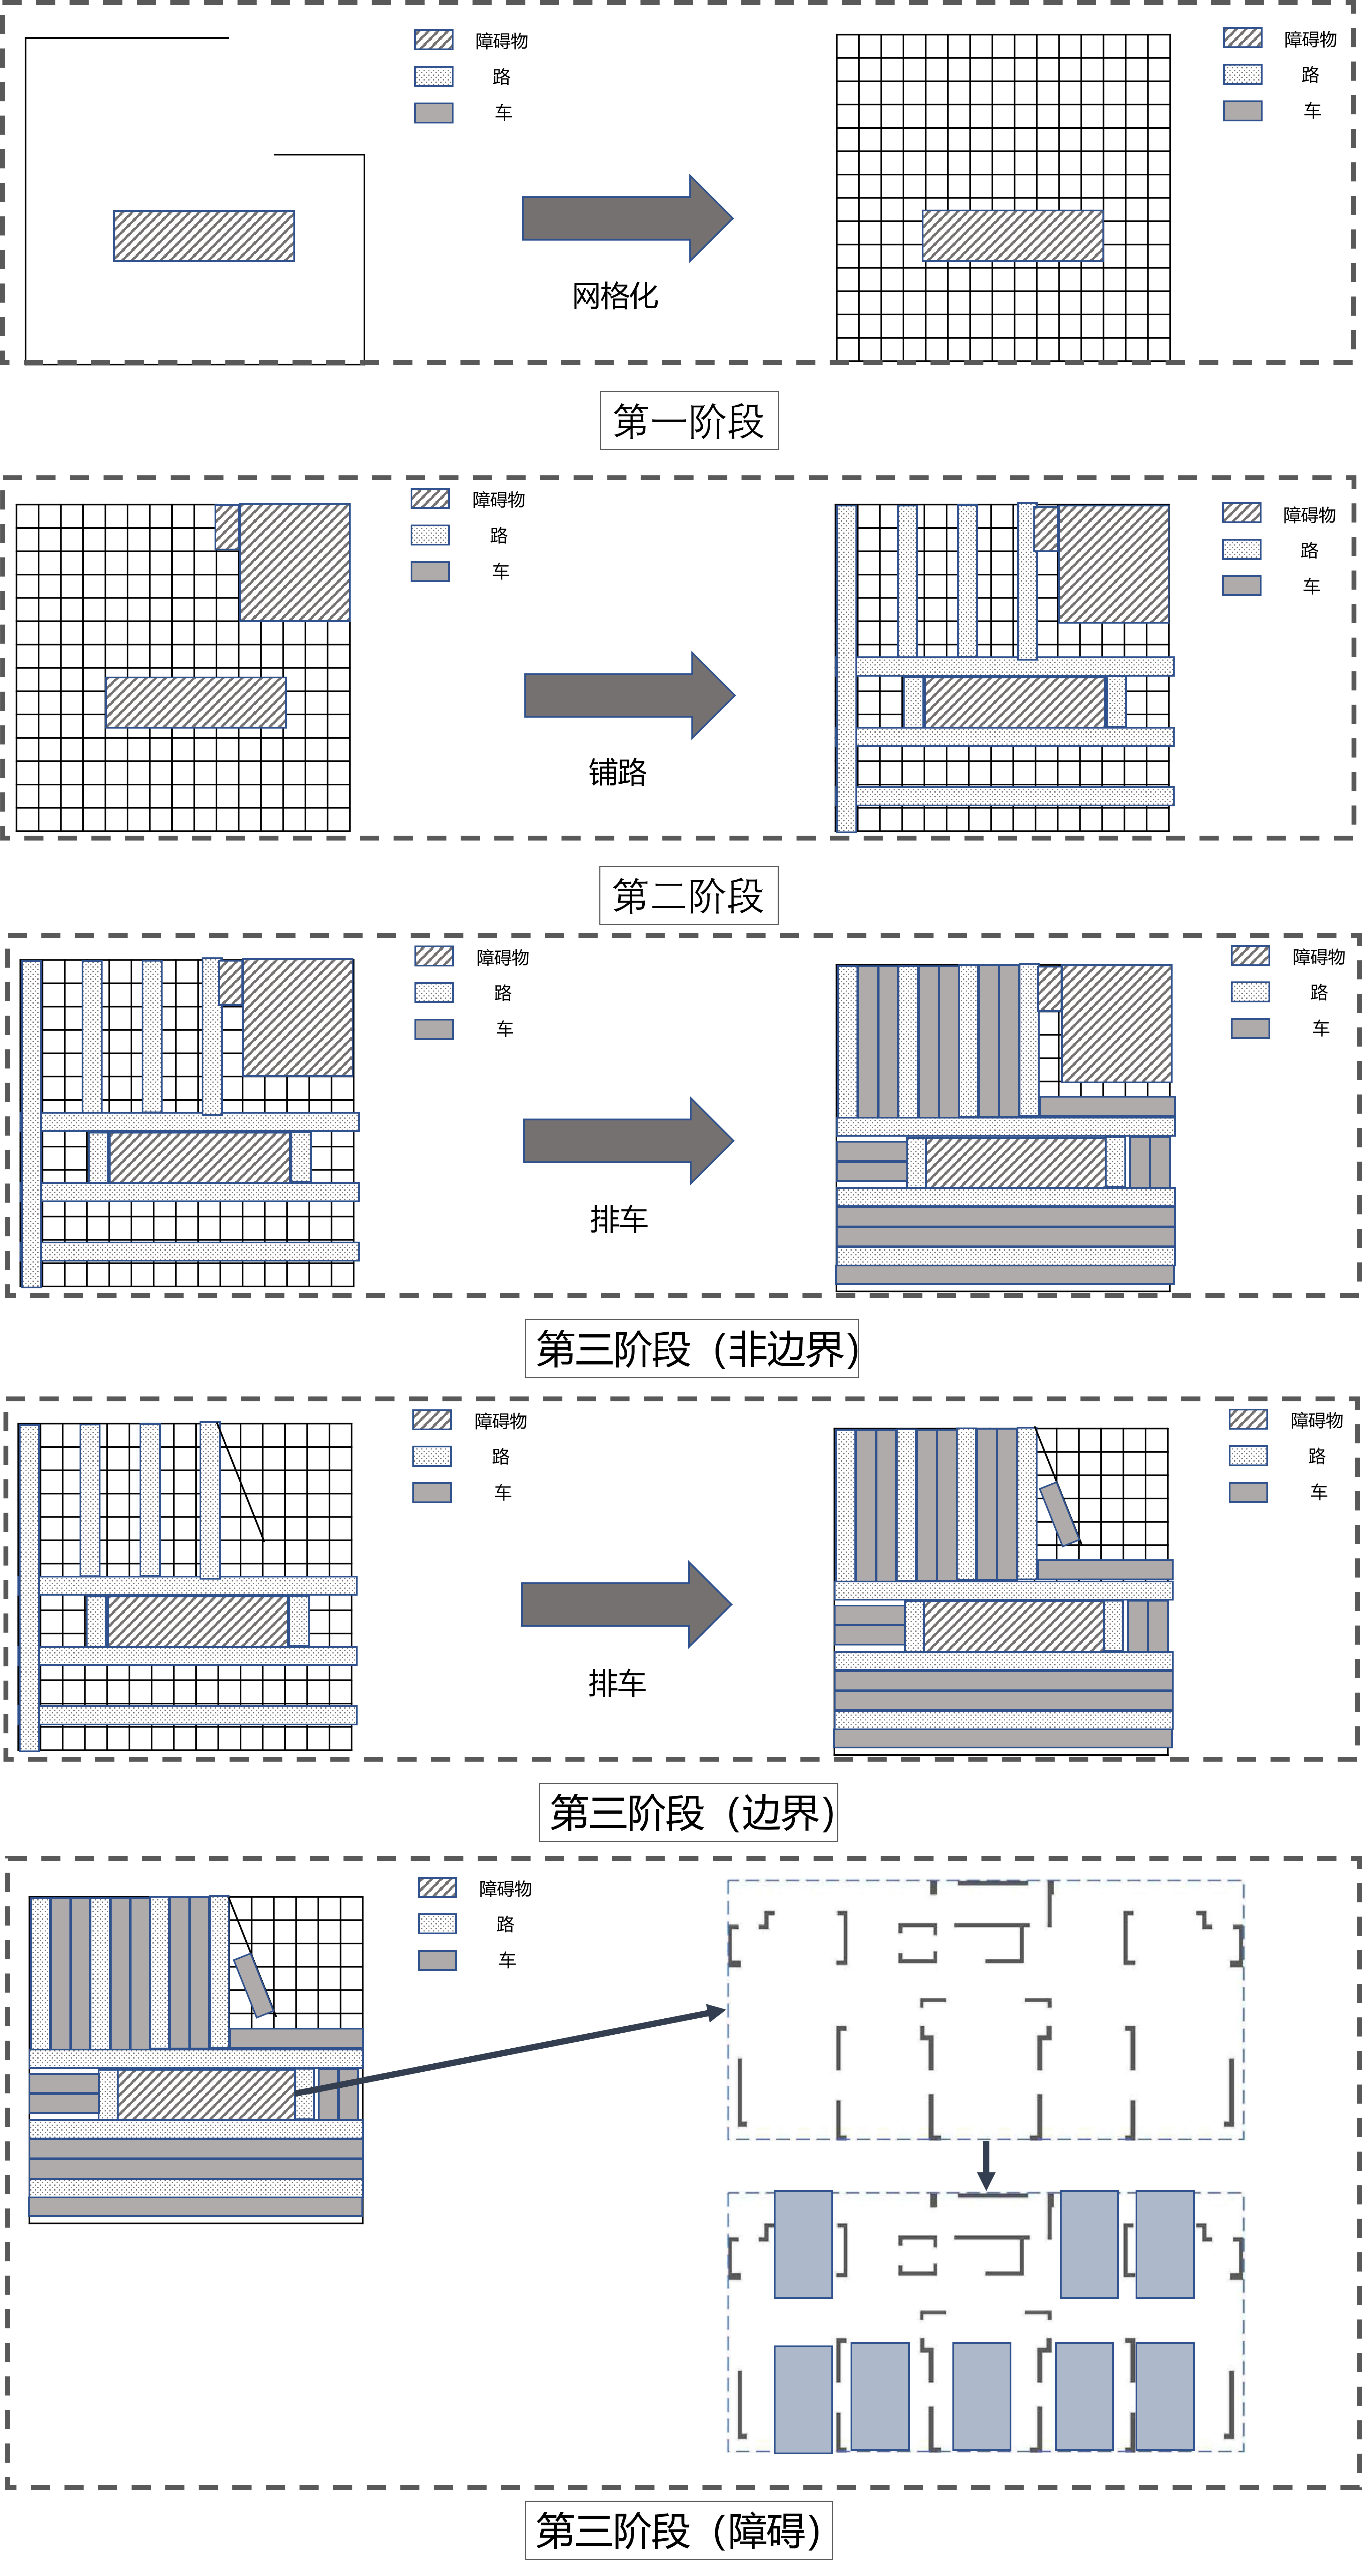
\includegraphics[width=0.7\textwidth]{pictures/技术路线/技术路线_改.png}
  \caption{技术路线图}
  \label{fig:tec_road}
\end{figure}
\subsection{工具选型}
\subsubsection{Pytorch}
PyTorch是一款基于Python的库,以其在科学研究、教育和工业界广泛应用的深度学习框架而闻名。它提供了基于数组的编程模型,通过GPU加速实现微分功能,并与Python生态系统中的自动微分紧密集成。同时,PyTorch自然地与标准绘图、调试和数据处理工具集成,采用命令式编程模型。支持与外部库双向交换数据,用户可以根据项目需求或性能要求自由更换组件。PyTorch实现了张量数据结构、GPU和CPU操作符以及基本的并行原语。它的自动微分系统包括对大多数内置函数的梯度计算,具有立即执行动态张量计算的能力,性能上与当前最快的深度学习库相媲美,在研究社区中备受欢迎(如2019年ICLR提交的296篇论文中提到的\cite{paszke2019pytorch})。

在本项目中,我们选择使用Pytorch实现自定义的深度学习模型,并便捷地处理高维输入输出,同时利用分布式训练在多个GPU上并行训练,为项目实现提供了高效可靠的解决方案。
\subsubsection{pyautocad}
pyautocad\cite{shahzad2023implementing}是一款专注于与AutoCAD软件交互的Python库,通过AutoCAD的COM接口实现对AutoCAD对象模型的访问和操作。具有多版本支持、执行AutoLISP代码的功能,其直观且方便的API设计使得通过Python直接调用AutoCAD的对象和方法变得简便。尤其适用于需要自动化处理CAD图纸的项目,拥有丰富的社区支持和文档资源,为开发人员提供了可靠的工具。

在本项目中,pyautocad通过利用与AutoCAD的强大交互能力,高效地实现对CAD图纸的自动修改和处理,也便于生成后的进一步修改。pyautocad为项目提供了便捷而可靠的解决方案,使得与AutoCAD集成的开发变得更加顺畅。
\subsubsection{AutoCAD}
AutoCAD是一款由AutoDesk公司开发的计算机辅助设计(CAD)软件,广泛应用于建筑、土木工程、机械设计等领域。它提供了强大的绘图和建模工具,允许用户创建、编辑和分析二维和三维设计。AutoCAD支持多种文件格式,包括DWG,使其成为设计领域的行业标准之一。其用户友好的界面和丰富的功能集使得设计师能够高效地进行各种设计任务,从简单的图纸绘制到复杂的建筑模型。

在该项目中,AutoCAD提供了强大的绘图和建模工具,通过对于绘制在AutoCAD中图纸,使得设计师能够轻松编辑并更改生成后的图纸。其支持DWG格式的特性也确保了设计图的广泛可用性。此外,AutoCAD的灵活性和可扩展性使其能够与其他工具和编程语言进行集成,如通过pyautocad连接Python脚本,实现与算法代码的交互。这种整合为项目提供了便捷的工具,使得设计和修改车库布局更加直观、高效。AutoCAD在车库设计项目中的应用为设计师提供了一个全面的平台,满足各种设计需求,从而提高了设计效率和质量。
\subsection{可行性分析}
\subsubsection{理论可行性}
随着机器学习的进步,我们能够利用这些深度学习、进化策略\cite{1020332216.nh}等方式来提高地库排布的智能性或者加快排布速度。许多研究证明在处理地库排布问题时,机器学习的应用是十分有效的,并为本研究提供了扎实的基础,保证了最终实现的成功率和可靠性,因此利用机器学习实现地库排布存在理论可行性。
\subsubsection{经济可行性}
在本课题的研发过程中,不需要使用额外的数据集,因此在收集数据方面不需要开销。而且模型训练与评估所需的GPU可由导师实验室提供,项目开发成本较低,因此在经济方面具有可行性。
\subsubsection{应用可行性}
市面上存在许多车位排布的软件,但应用技术不同,有些对于斜边、不规则图形的处理较为简单,在该项目中可对这些特殊情况进行处理,因此,该项目在应用上具有较高的可行性。
\subsection{研究思路}
\subsubsection{地下车库排布的算法与实现}
在解决地下车库设计的复杂问题中,我们需设计一种基于强化学习的车位排布算法。这一算法的关键目标是在考虑地下车库边缘为不规则形状、内部存在空洞的情况下,划分出更多的车位,同时确保车辆行驶的便利性,以满足实际地库的需求。这一步骤需涉及问题模型建立、地库主路铺设方式、车位排布算法这三大部分。

{\bfseries 问题模型建立:}
由于针对的图纸可能具有不规则的边界,因此直接处理起来较为繁琐。为了简化处理流程,我们采用了对初始图纸进行网格化的方法。以道路宽度为基准,将图纸划分为小方格,每个方格具有5种不同状态,分别表示边界外、障碍、空地、道路和车位,对应于-2、-1、0、1、2。在处理过程中,如果格子位于空地和边界外区域的交界或者空地和障碍的交界,则该区域被处理为边界外或者障碍。特别是在处理障碍时,我们将集中的障碍划分为同一障碍区域,并取所有障碍中的最大和最小xy值计算得到边界坐标,以便更清晰地定义障碍区域,并方便地进行后续处理。

{\bfseries 地库主路铺设方式:}
如何在机器学习这一庞大范围内选择合适的算法铺设主路是需要解决的问题。机器学习是一种人工智能的分支,致力于研究如何通过让计算机从数据中学习并改善性能,实现对任务的自动化处理。这一领域的核心思想是通过训练模型,使其能够自动发现数据中的模式,从而做出预测或决策。比较不同的机器学习算法我们发现:
\begin{itemize}
    \item {\bfseries 监督学习:}要大量的标记数据,而在车位规划中,获取大规模标记的停车数据可能会非常昂贵且困难;同时,监督学习不适用于动态环境,若停车环境是动态的,由于它只能学习已知标签的模式,因此可能无法很好地适应变化。
    \item {\bfseries 无监督学习:}生成的模型可能难以解释,因为它通常是从数据中找到的模式,而非直接关联到标签或奖励;并且,它通常是用于探索性分析,可能无法满足特定的停车规划需求。
\end{itemize}

相比于前两种学习方式,强化学习适用于智能体与环境交互、学习和改进策略的情境,因此对于车位规划中道路、车位、障碍等的交互而言,它是一种自然的选择,与此同时,强化学习还能够考虑到长期奖励,对于车位规划这样的任务,这意味着模型可以学到更智能、长远的停车策略,还有一点就是,强化学习在适应动态环境方面表现良好,可以通过不断与环境交互来优化策略。

在实际应用中,选择强化学习的优势在于它能够适应车位规划这类需要智能体与环境交互、学习和优化策略的场景,同时能够考虑到长期奖励,从而生成更智能、适应性更强的停车决策模型。

强化学习主要包括智能体、环境、行为、奖励和状态这几个部分。
\begin{figure}[H]
  \centering
  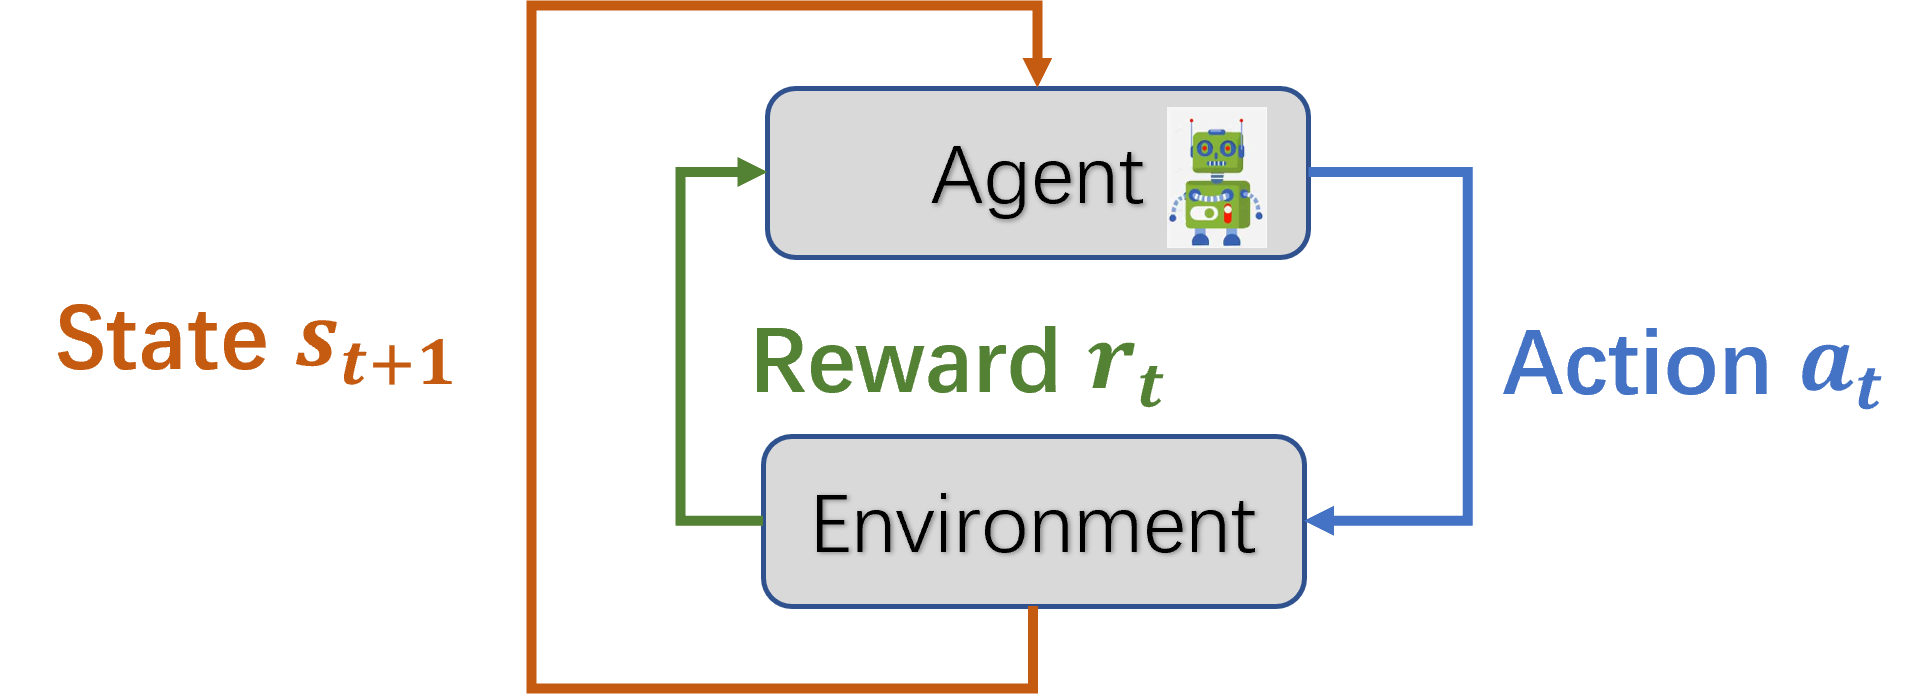
\includegraphics[width=0.7\textwidth]{pictures/强化学习.png}
  \caption{强化学习基础组成}
  \label{fig:reinforcement_learning_component}
\end{figure}
在车位排布中,智能体的任务是铺路;环境是第一步建立的状态矩阵,可以用不同的数字进行标记并区分;行为则是直走、向左走和向右;状态指所在单元格的数字标记对应的状态;奖励在铺路过程中是不进行计算的,而是在车位排布完之后,通过比较分值大小,对整个车库进行评估。其中奖励计算主要包含两个部分,分别为车辆数和交通。车辆数就是计算该图纸中的车位总数;交通则是通过三个指标来进行度量,分别为道路密度、连通性和便捷度,具体公式如下:
\begin{equation}
  R=n*S_{car}/S_{sum}+w*Traffic,\label{reward}
\end{equation}
\begin{equation}
  Traffic=\frac{1}{3}*(T_{density}+T_{connectivity}+T_{convenience}),\label{reward_traffic}
\end{equation}
\begin{equation}
  T_{density}=\frac{Length(path)}{Area(land)},\label{reward_traffic_density}
\end{equation}
\begin{equation}
  T_{connectivity}=\frac{\sum_{dot \in dots}\mathbbm{1}[Degree(dot)=2]'}{Num_{dots}},\label{reward_traffic_connectivity}
\end{equation}
\begin{equation}
  T_{convenience}=\frac{\sum_{dot \in dots}{Length(shortest\_path(dot))}}{Length(path)},\label{reward_traffic_convenience}
\end{equation}

其中$T_{density}$表示道路密度,$T_{connectivity}$表示道路连通性,$T_{convenience}$表示最短环路,$Length(path)$表示道路总长,$Area(land)$表示土地面积,$dots$表示图上除去边界外和障碍的点,$Num(dots)$表示点的个数,$shortest\_path(dot)$表示最短环路。

由于最终排布结果取决于奖励的大小,因此该模型不需要大量的数据集。相较于数据集这一概念,在我们的项目中主要还是需要不同的图纸和与之对应的具对比意义的基准数据,从而帮助判别模型的合理性。

{\bfseries 车位排布算法:}
车位排布算法根据区域不同,主要分为三大模块,分别为非边界区域、边界区域、障碍物矩形闭包区域三大部分,具体描述如下:
\begin{itemize}
  \item {\bfseries 非边界区域内的车位排布算法:}
  非边界区域的车位排布,我们基于前一步骤得到的道路信息,主要利用车位组的概念进行辅助铺设。具体而言,我们对所有非边界区域的空地上分割为许多矩阵,通过基于贪婪算法进行最小矩阵合并。每次引入一个区域,通过将矩阵区域进行递归合并铺设,找出最大车位数量的矩形合并组合,其中每个矩形需满足大于可放入一个车位。通过这种方式,我们将最大化地利用停车位,确保在有限的空间内划分出尽可能多的车位。
  \item {\bfseries 边界区域的车位排布算法:}
  针对边界区域,若其中能放置多排车位,我们会进一步将其分割为两个部分,内部按照非边界区域进行分割,剩下则为新的边界区域。针对边界区域,为了兼顾便捷度和空间利用,我们选择将车位沿着斜边进行放置。同时考虑到障碍物的存在可能会导致距离边界的距离不足以排布对应类型的车位,因此基于王潇霆\cite{1023719817.nh}等人的研究,可以通过增加$45^{\circ}$和$30^{\circ}$和$60^{\circ}$等模块的方式增加车位数量,用进化算法进行边界区域车位的排布。
  \item {\bfseries 障碍物矩形闭包区域的车位排布算法:}
  对于障碍物矩形闭包中的空地进行处理是车库设计中的重要一环。我们的目标是设计一种算法,能够在闭包区域最大化排布车位,同时满足障碍物矩形内外的交通连通性要求。基于冯嘉宇\cite{1022674189.nh}等人的研究,我们沿着障碍物闭包的边缘进行计算可排布区域。我们将进一步根据相邻情况进行分类,分别考虑相邻为边界或是车位的不同情况。若相邻为边界,则需向外空出一个车位;若相邻为车位,则需比较内外车位个数的多少,从而选择更优的策略。
\end{itemize}
\subsubsection{地下车库排布的可视化}
可视化操作在车库设计中扮演着至关重要的角色,它不仅有助于设计师直观地比较不同算法的效果,还为他们提供了一个便捷的工具,以更直观的方式参与车库设计的过程。通过将算法生成的车位排布图以可视化的形式呈现,设计师能够迅速识别设计中的优点和不足,并进行必要的修改以满足特定需求。

在实现地下车库排布的可视化过程中,pyautocad被用来连接AutoCAD和算法代码。具体为以下几步:

{\bfseries 调用pyautocad进行可视化转换:}利用pyautocad的API,将算法生成的地下车库数据转换为AutoCAD中的设计图。通过调用pyautocad提供的方法,可以在AutoCAD软件中创建图层、绘制车位、标记道路,以及呈现其他相关设计元素等。

{\bfseries 实时更新设计图:}在数据转换的过程中,通过pyautocad与AutoCAD的实时交互,确保设计图的即时更新。这使得在算法生成数据发生变化时,设计图能够及时反映这些变化。

{\bfseries 保存设计图和结果:} 一旦设计图的生成完成,通过pyautocad将结果保存为AutoCAD支持的文件格式,如DWG。这样,生成的地下车库设计图可以随时被打开和查看。

综上,使用pyautocad实现连接AutoCAD和算法代码,将地下车库数据可视化为AutoCAD中的设计图,实现了从算法生成到CAD图形可视化的无缝转换。这种连接方式提高了设计效率,同时确保了设计图的准确性和实时更新。
\subsubsection{比较常见强化学习并验证}
在选择适合地下车库排布问题的强化学习算法之前,我们将从理论角度对比各个常见的强化学习算法,包括但不限于深度Q网络(DQN)、引入RNN的深度Q网络(DRQN)等。通过分析它们的特点,我们将能够综合选择适用于该场景的算法。

在验证阶段,我们将使用已验证过的图纸进行实际校验,考察各个算法在不同铺路情况和收敛速度等方面的性能表现。通过这一过程,我们将得到各个算法的实际效果,并最终进行全面对比,为选择最适用于地下车库排布问题的强化学习算法提供科学依据。
\subsubsection{评估算法指标并与现有研究比较}
为验证我们新提出的车位排布方法的有效性,我们将制定有参考性的对比评价指标,例如车位数、平均出库时间、车位排布速度等。通过使用现有算法验证过的图纸进行校验,我们将能够验证我们的算法相较于其他现有模型在地下车库排布问题上的优越性。

同时,我们将对新算法与现有研究算法进行深入研究与比较。通过全面评估它们在各项指标上的表现,包括但不限于效率、准确性和实用性,我们将能够更全面地了解这些算法的优劣势。这一比较将为实际应用中的决策提供可靠的参考依据,确保所选算法能够在各方面胜任实际场景中的挑战。
\subsection{非技术因素}
{\bfseries 法律方面:}非技术因素中涉及的主要是法律法规的问题。针对软件的应用方面,本项目仅用于个人学习与研究,不涉及商业应用,没有侵犯其他软件的合法权益,也没有违反相关法律法规。我们在使用AutoCAD软件\cite{JCJG202304039}时遵循了教育许可方案,并保证在使用和开发的过程中不会侵犯AutoCAD的版权和专利权。与此同时,设计时的车位、道路大小以及柱网排布等尺寸均按照法律法规来进行设计。但消防等更为详细的设施需要,可能需要在进一步在设计图展示在AutoCAD之后,由设计师进行调整。这些设计参数的合规性将有助于确保地下车库的建设和使用在法律法规框架内,保障人员生命财产安全,同时也有利于项目的可持续发展。

{\bfseries 数据隐私和安全:}强化学习中涉及的数据只有现成,互联网上可见的设计图纸,均不涉及到个人隐私。本项目考虑并遵守相关的数据隐私法规,采取措施保护用户数据的安全性。

{\bfseries 结构安全和承重考虑:}地下车库的建设需要充分考虑地上结构的安全和承重能力。在设计车库时,需要确保地下结构不会对地上建筑物的承重结构造成不利影响。这涉及到合理的承重分布和结构设计,以防止地下车库的建设对地上建筑物的稳定性产生负面影响。
\subsection{预期研究成果}
{\bfseries 一种强化学习的地下停车库车位排布的算法:}我们期望提出一种创新的、基于强化学习的地下停车库车位排布算法。该算法将能够有效应对不规则形状以及内部空洞等情况,确保生成的车位布局既满足最大化停车容量的需求,又保障车辆行驶的便利性。

{\bfseries 基于强化学习的地下停车库车位排布算法的AutoCAD绘制:}通过与AutoCAD软件的连接和控制,我们将实现对基于强化学习的地下停车库车位排布算法生成结果的直观可视化。通过调用pyautocad的API来实时更新设计图,最终将生成结果保存成设计图。

{\bfseries 对常见强化学习进行研究与验证:}
通过深入研究和验证常见的强化学习算法,我们将得出针对地下停车库排布问题的最佳选择。理论分析和实验验证将为我们提供对各算法性能的深刻理解,为最终选择提供科学依据。这将是一个可迁移、可拓展的研究成果,有望在其他类似问题中具有指导意义。

{\bfseries 对现有研究算法进行研究与比较:}
通过对现有研究算法的深入研究和全面比较,我们将评估它们在地下停车库排布问题上的优劣。通过对比新提出算法与现有算法的性能,我们将验证新算法的相对优越性。这一研究成果将为实际应用中的决策提供科学依据,确保所选算法能够胜任实际场景中的挑战。
\section{研究工作计划}
\begin{longtblr}[
    theme=plain,
    entry=none,
  ]{
    colspec = {|X[2,l]|X[3,l]|},
    row{1} = {c},
    hlines
  }
    起止时间 & 内容 \\
    2023.11.05-2023.12.10 & 查阅文献、撰写文献综述、外文翻译 \\
    2023.12.11-2024.1.8 & 确定研究内容、撰写开题报告 \\
    2024.1.9 & 开题答辩 \\
    2024.1.10-2024.1.31 & 行为、环境、奖励等的设计 \\
    2024.2.1-2024.2.29 & 不同车位规划模型的学习与训练 \\
    2024.3.1-2024.3.14 & 不同车位规划模型的对比与评估 \\
    2024.3.15 & 中期检查 \\
    2024.3.16-2024.4.18 & 整理上述工作并完善论文 \\
    2024.4.19-2024.4.22 & 教师评阅 \\
    2024.4.23-2024.5.16 & 学生进一步修改完善毕业设计 \\
    2024.5.17 & 毕业设计第一次答辩 \\
    2024.5.18-2024.5.23 & 学生进一步修改完善毕业设计 \\
    2024.5.24 & 毕业设计第二次答辩 \\
  \end{longtblr}
  